% Copyright 2010 by David Pfau

\documentclass[16pt]{beamer}
\usepackage{algorithm}
\usepackage{algorithmic}
\usepackage{natbib}

% Setup appearance:

\usetheme{Dresden}
%\usetheme{Copenhagen}
\usefonttheme[onlylarge]{structurebold}
\setbeamerfont*{frametitle}{size=\normalsize,series=\bfseries}
\setbeamertemplate{navigation symbols}{}

% Standard packages
\usepackage[english]{babel}
%\usepackage[latin1]{inputenc}
%\usepackage{times}
%\usepackage[T1]{fontenc}
%\usepackage{nnfootnote}
\usepackage{amsfonts}
\usepackage{amsmath}
%\newcommand{\argmax}{\operatornamewithlimits{argmax}}
\def\newblock{\hskip .11em plus .33em minus .07em}
% Setup TikZ

%\usepackage{tikz}
%\usetikzlibrary{arrows}
%\tikzstyle{block}=[draw opacity=0.7,line width=1.4cm]


% Author, Title, etc.

\title[Probabilistic Deterministic Infinite Automata] 
{
	Probabilistic Deterministic Infinite Automata
}

\author[D. Pfau, N. Bartlett, F. Wood]
{
  David~Pfau %\inst{1}
}

\institute[Columbia]
{
  %\inst{1}%
  Columbia University
}

\date[Poster T81]
{8 December 2010}

%\def\blfootnote{\xdef\@thefnmark{}\@footnotetext}

% The main document

\begin{document}

\begin{frame}
	\begin{block}{Discrete Sequence Modeling}
		\begin{itemize}
			\item{01101010111001011...}
			\item{CGTAACCGATTAC...}
			\item{\em Four score and seve...}
		\end{itemize}
	\end{block}
	\begin{block}{Tasks}
		\begin{itemize}
			\item{Conditional Prediction}
			\item{Typicality - Clustering, etc}
		\end{itemize}
	\end{block}
\end{frame}

\begin{frame}
	Choose model that trades off accurate prediction, space complexity and prediction speed: {\em Probabilistic Deterministic Infinite Automata} 
	\begin{center}
		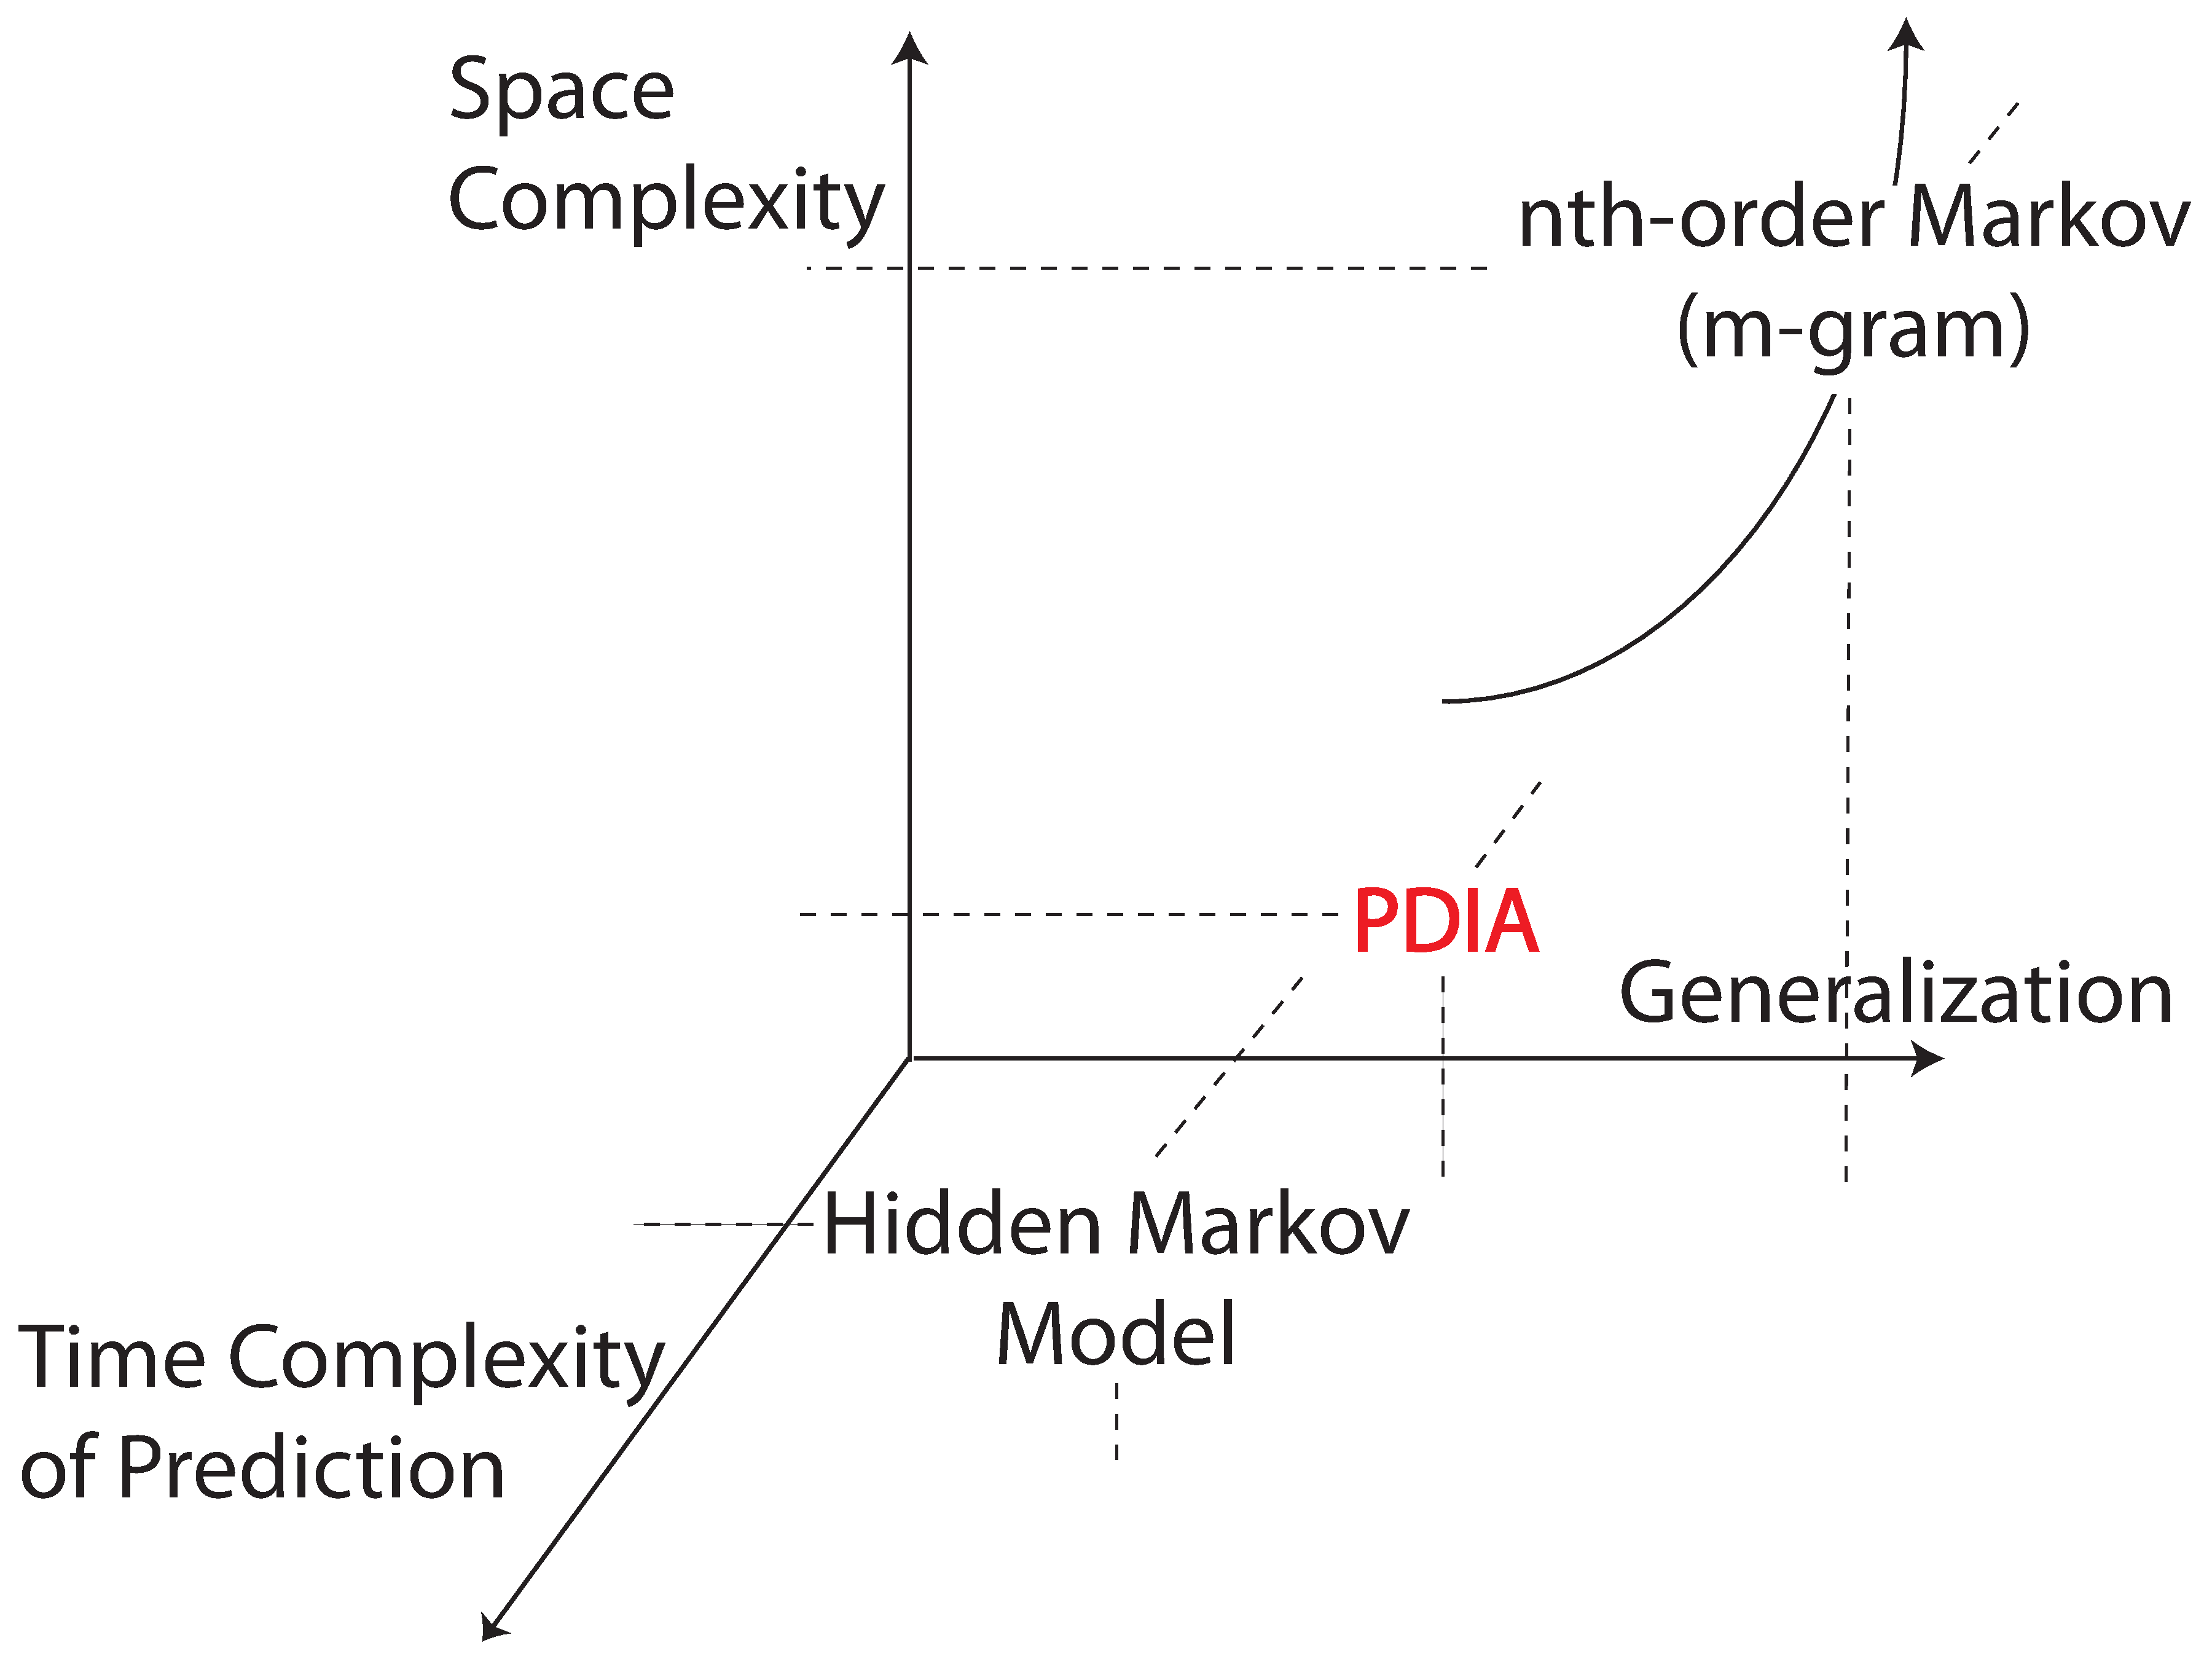
\includegraphics[scale=0.1]{plot.pdf}
	\end{center}
\end{frame}

\begin{frame}
	\begin{columns}[top]
		\column{0.5\textwidth}
			\begin{block}{Probabilistic DFA}
				\begin{itemize}
					\item{Roughly: HMMs with one possible path through states given data}
					\item{m-gram $\subsetneq$ PDFA $\subsetneq$ HMM}
				\end{itemize}
			\end{block}
			\begin{block}{An Infinite Automata Prior}
				\begin{itemize}
					\item{Define Prior over DFA topology}
					\item{Biased towards small DFA that reuse states}
					\item{Let bound on state cardinality $\rightarrow \infty$}
				\end{itemize}
			\end{block}
		\column{0.5\textwidth}
			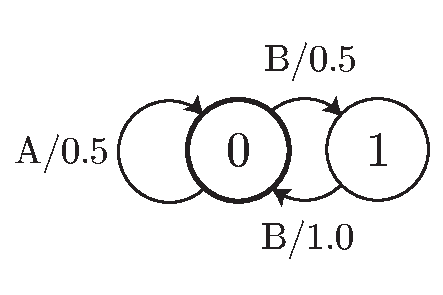
\includegraphics[scale=0.8]{even.pdf}
	\end{columns}
\end{frame}

\begin{frame}
	\begin{block}{Results}
		\begin{itemize}
			\item{Recovers topology of artificial PDFAs}
			\item{Natural language: generalizes as well as 3rd-order Markov, 1/10th the model size}
			\item{Averaging predictions over DFA topologies better than single topology}
		\end{itemize}
	\end{block}
	\begin{block}{Recap}
		\begin{itemize}
			\item{Nonparametric Bayesian learning of simple models for discrete sequences}
			\item{Favorable tradeoff between model size and generalization}
			\item{Faster forward prediction than for HMM}
		\end{itemize}
	\end{block}
\end{frame}

\end{document}